% !TeX root = ../main.tex

%\section{Killer Whale Case Study}

The CarHHMM-DFT was used to analyze dive data from a northern resident killer whale off the coast of British Columbia, Canada. Acceleration data can be a good proxy for energy expenditure \citep{Green:2009}, but studies suggest that the behavioral state must be taken into account when using accelerometer data \citep{Dot:2016}. Therefore, understanding both the behavioral state of the killer whale as well as the distribution of accelerometer data within each behavioral state is import to understand the energetic requirements of killer whales. This in turn can assist conservation efforts.

\subsection{Data Collection and Preprocessing}

The data used in this study was collected on September 2, 2019 from 12:49 pm to 6:06 pm and consists of depth and acceleration in three orthogonal directions. Observations were collected at a rate of 50 hertz. Tagging the killer whale caused anomalous behavior before 1:20 pm and after 6:00 pm, so observations in this time range were ignored. In addition, the tagging technology dropped data between 2:25pm and 2:37pm as well as between 4:07 and 5:07 pm, so any partially observed data within this time range were ignored as well. A killer whale ``dive" is considered to be any continuous chunk of data that occurs below 0.5 meters in depth and lasts for at least 10 seconds. Accelerometer and depth data were smoothed by taking a moving average with a window of 1/10th of a second. Data preprocessing was done in part with the \textit{divebomb} package in Python \citep{Nunes:2018}. After preprocessing the raw data, a total of 267 dives were observed. A plot of the raw data for all dives and a collection of five selected dives can be seen in (fig \ref{fig:data}) and (fig \ref{fig:data_one_dive}), respectively.

\begin{figure}[ht]
	\centering
	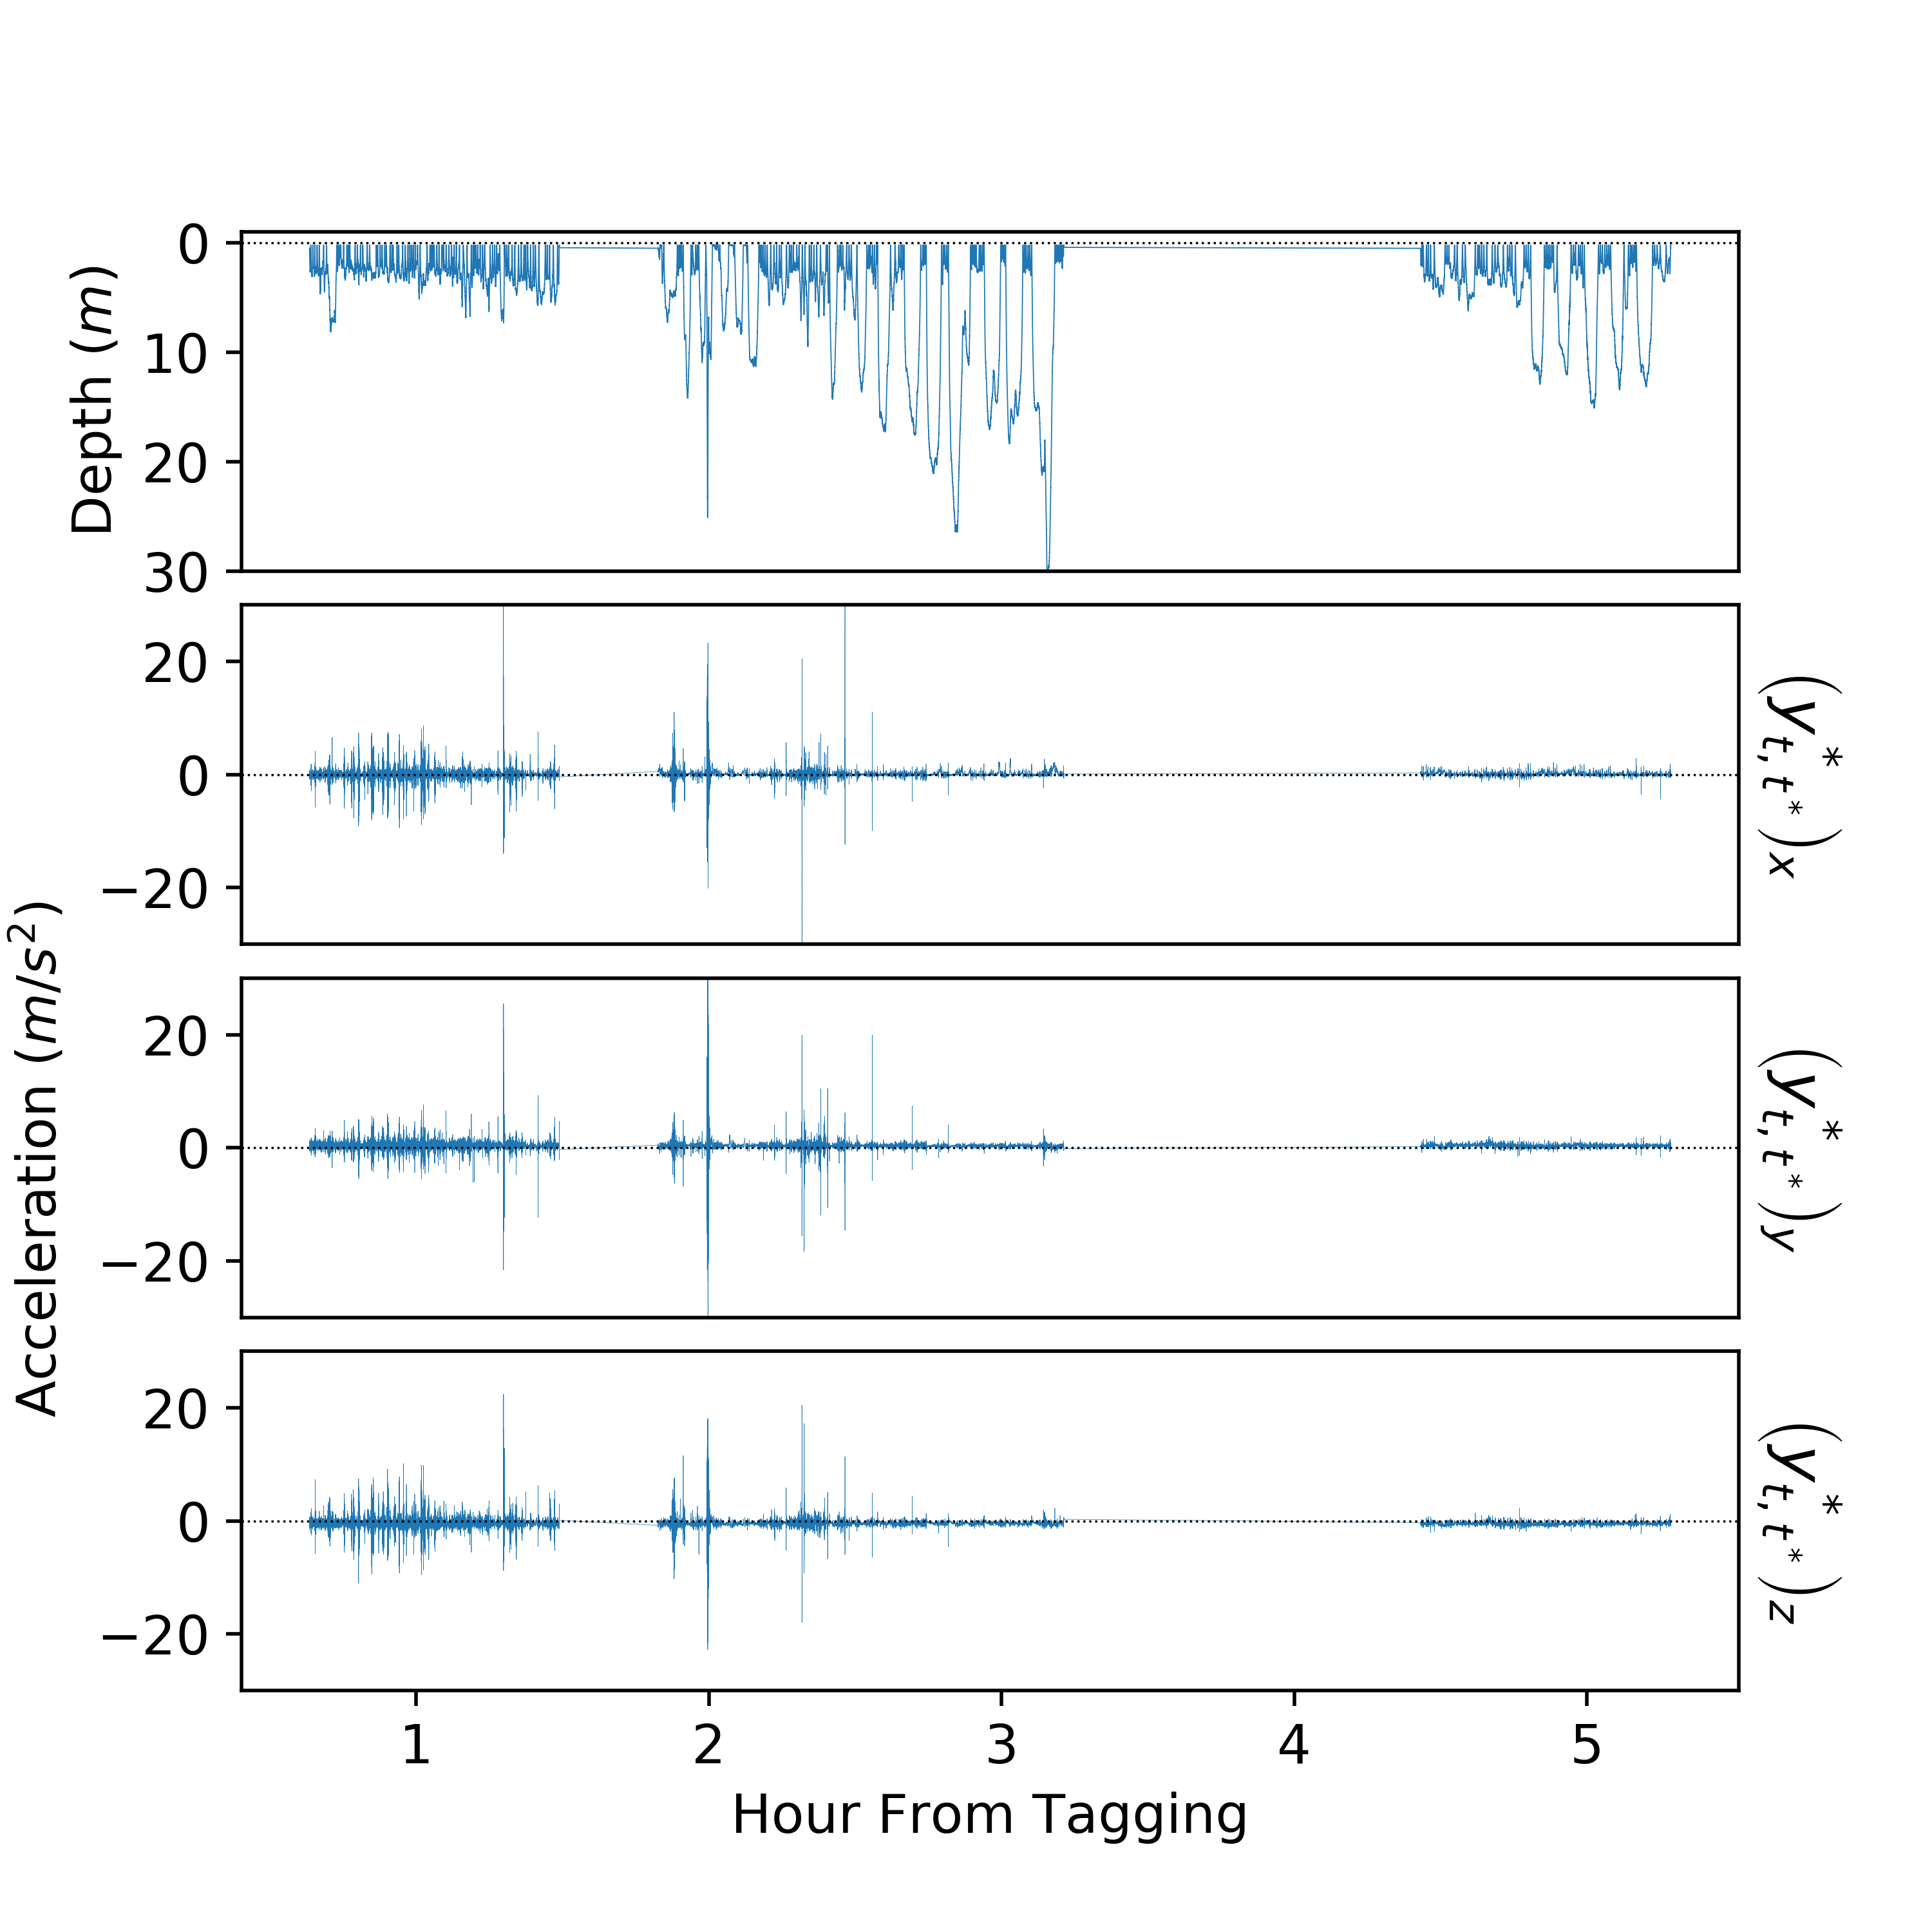
\includegraphics[width=5in]{../Plots/raw_data.png}
	\caption{Dive profile and Acceleration data of entire data set}
	\label{fig:data}
\end{figure}

\begin{figure}[ht]
	\centering
	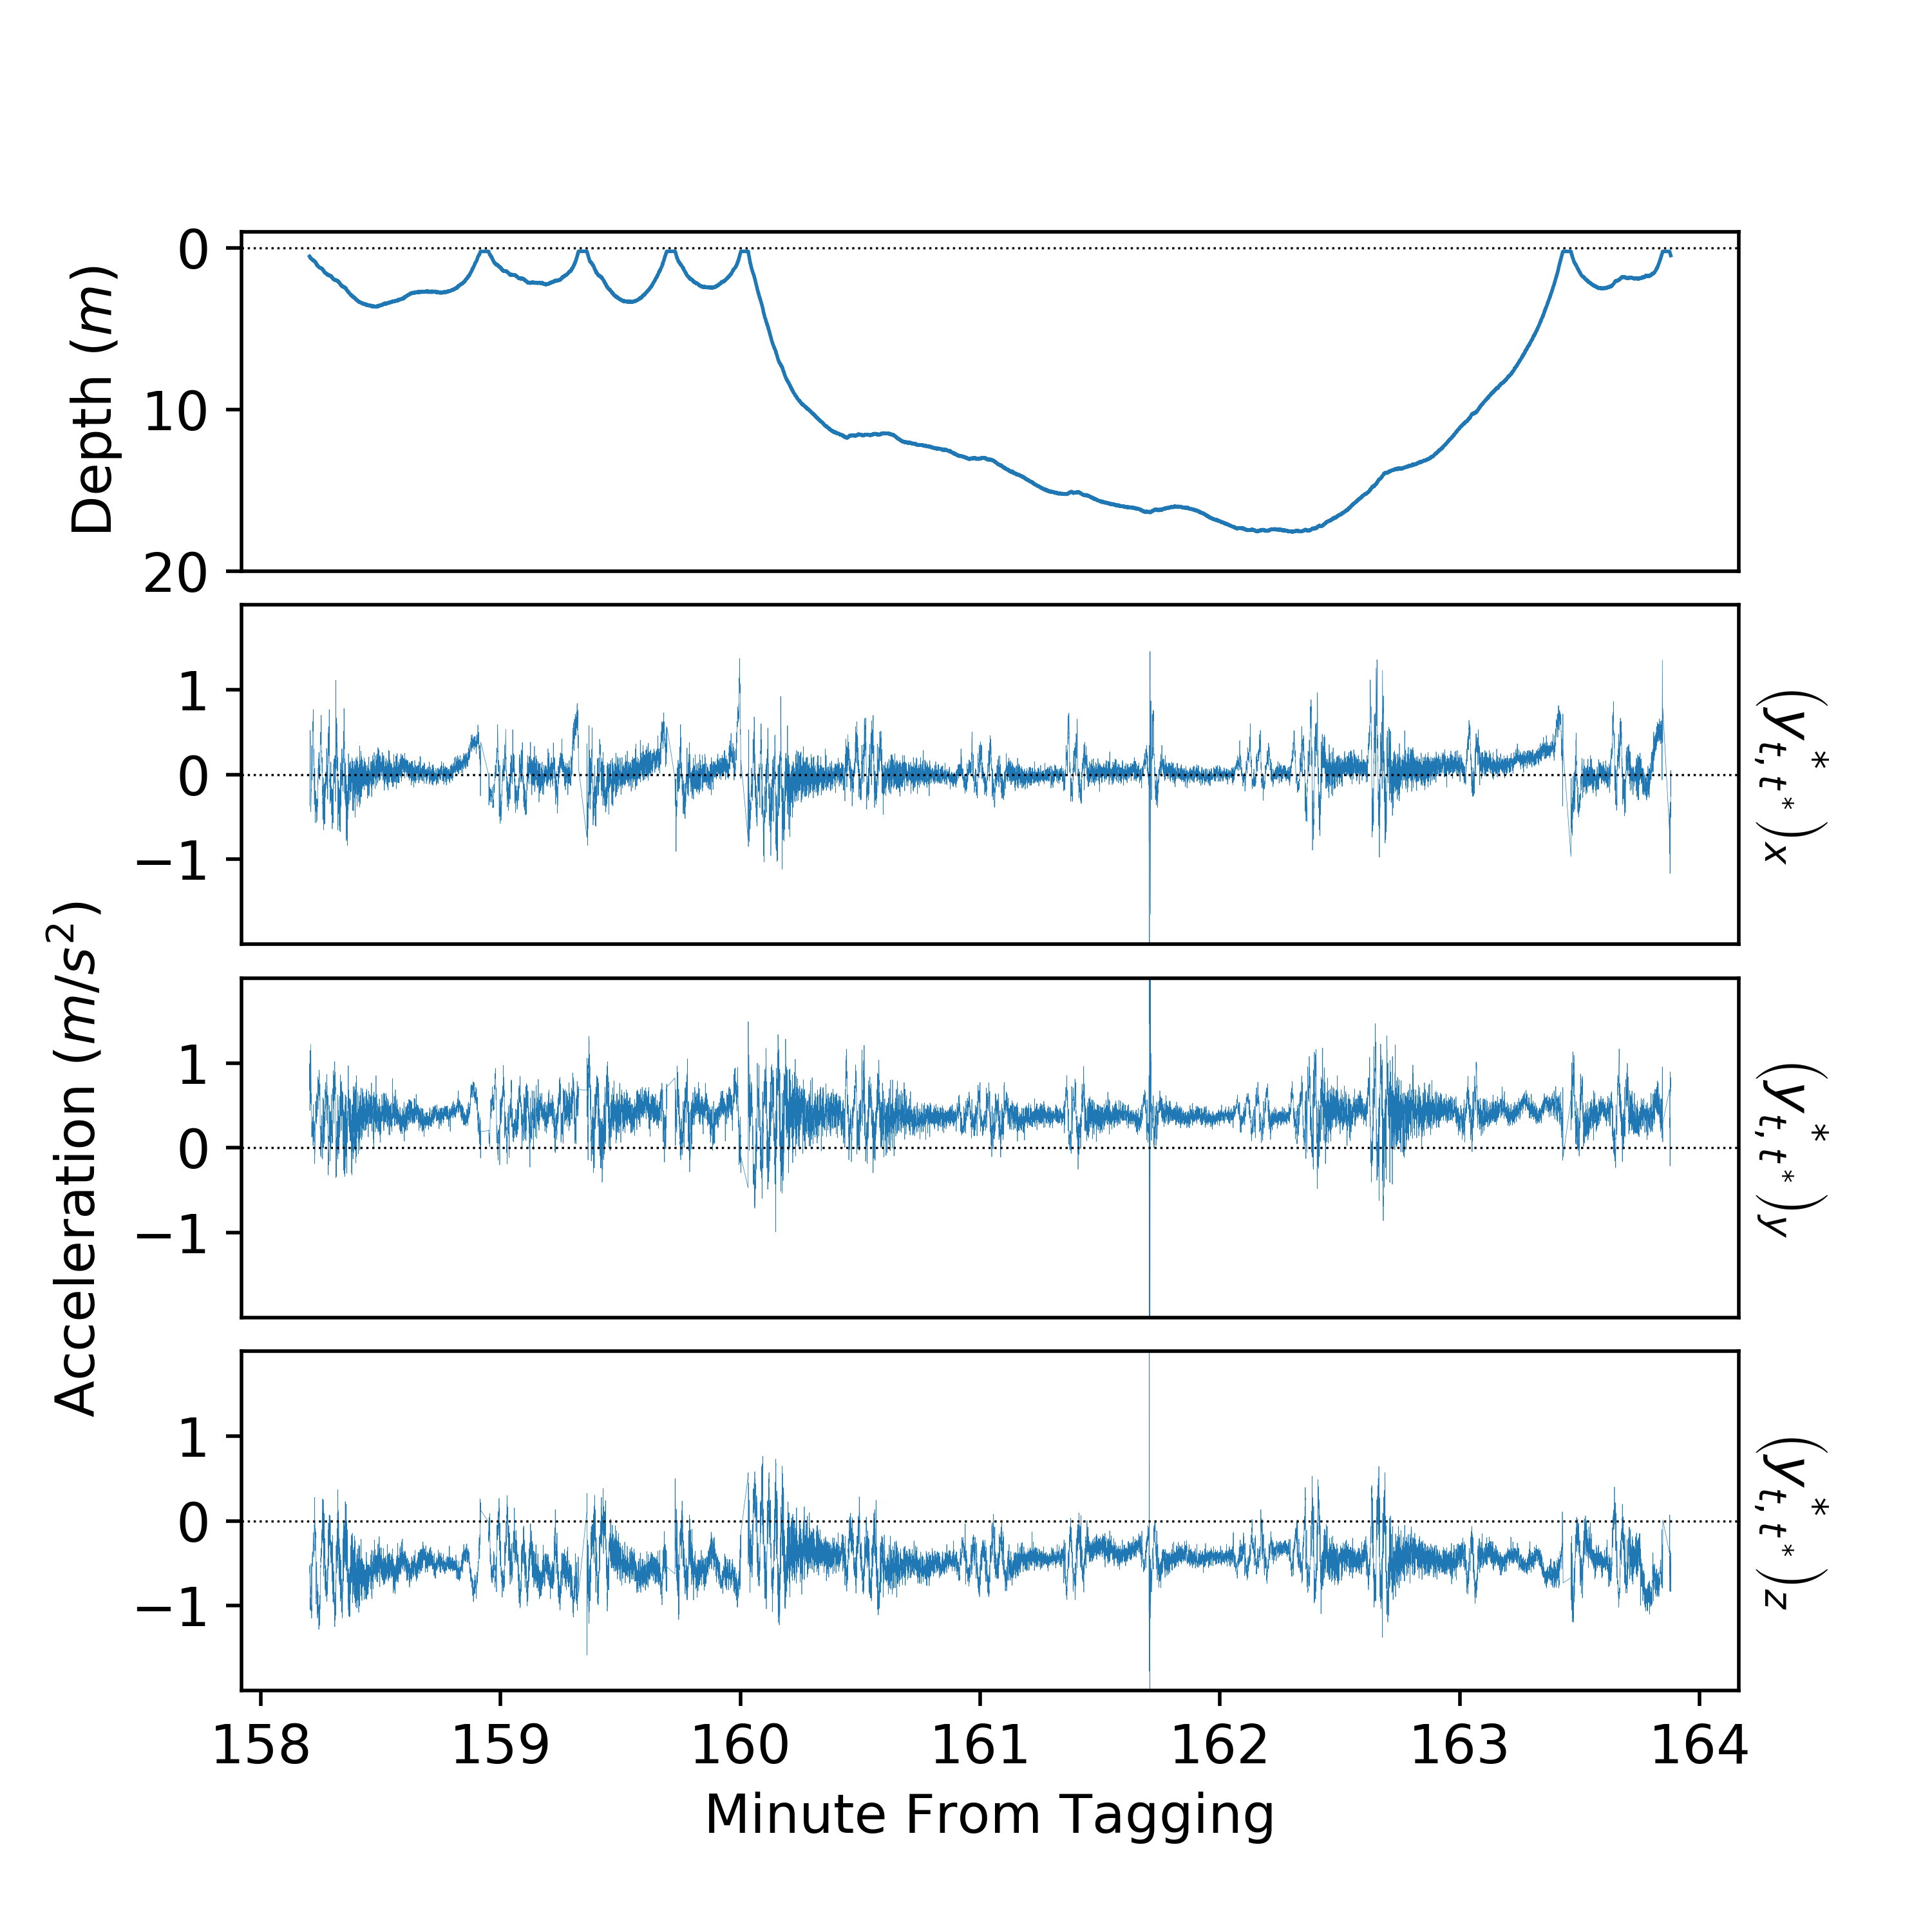
\includegraphics[width=5in]{../Plots/raw_data_5_dives.png}
	\caption{Dive profile and acceleration data for a collection of 5 dives of a killer whale.}
	\label{fig:data_one_dive}
\end{figure}

\subsection{Model Selection}

The coarse-scale observations were made up of the collection of dive durations in seconds, and the fine-scale observations were determined from the within-dive acceleration data. The dive durations $Y_t$ were assumed to follow a gamma distribution with unknown parameters $\{\mu,\sigma\}$:

$$\mathbb{E}(Y_t|X_t = i) = \mu^{(i)}$$
$$\mathbb{V}(Y_t|X_t = i) = \left(\sigma^{(i)}\right)^2$$

The acceleration exhibits significant sinusoidal behavior at several points in time (see fig \ref{fig:data_one_dive}), so the fine-scale observations $Z^*$ were made up of the DFT summary statistics of a two-second sliding window. Acceleration data was a 3-dimensional vector, so $Z^*$ was calculated as follows:
%
$$\mathbf{z}_{t,t^*}^{*(1)} := \mathcal{R}\left(\hat{\mathbf{y}}^{*(0)}_{t,t^*}\right) \qquad z_{t,t^*}^{*(2)} := \frac{1}{100}\sum_{k=1}^{10}||\hat{\mathbf{y}}^{(k)}_{t,t^*}||^2$$
%
$\mathbf{z}_{t,t^*}^{*(1)}$ is a 3-dimensional vector while $z_t^{*(2)}$ is a scalar. Summing the first 10 Fourier modes to calculate $z^{(2)}_{t,t^*}$ corresponds to a maximum frequency of $\tilde \omega = 5$ hertz. (Fig \ref{fig:lag}) displays a lag plot for all major features and reveals strong auto-correlation within $\mathbf{Z}^{*(1)}_{t,t^*}$ for all dimensions. Auto-correlation was therefore directly modeled into the the distribution of $\mathbf{Z}^{*(1)}_{t,t^*}$, which is assumed to be normally distributed with the following parameters:
%
$$\mathbb{E}(\mathbf{Z}^{*(1)}_{t,t^*}|\mathbf{Z}^{*(1)}_{t,t^*-1} = \mathbf{z}, X^*_{t,t^*} = i^*) = \phi_1^{*(i^*)} \mathbf{z} + (1-\phi_1^{*(i^*)}) \mathbf{\mu}_1^{*(i^*)}$$
$$\mathbb{V}(\mathbf{Z}^{*(1)}_{t,t^*}|\mathbf{Z}^{*(1)}_{t,t^*-1} = z,X^*_{t,t^*} = i^*) = \left(\mathbf{\sigma}_1^{*(i^*)}\right)^2 I_3$$
%
where $I_3$ is the identity matrix, $\phi_1^{*(i^*)} \in \mathbb{R}$, $\mathbf{\mu}_1^{*(i^*)} \in \mathbb{R}^3$, and $\mathbf{\sigma}_1^{*(i^*)} \in \mathbb{R}^3$.

While $Z^{*(2)}_{t,t^*}$ also exhibits some auto-correlation, the relationship is less strong, and the biological interpretation of auto-correlation within $Z^{*(2)}_{t,t^*}$ is unclear. For this reason, auto-correlation was not incorporated into the emission distribution of $Z^{*(2)}_{t,t^*}$. The distribution of $Z^{*(2)}_{t,t^*}$ was also assumed to be gamma:
%
$$\mathbb{E}(Z^{*(2)}_{t,t^*}|Z^{*(1)}_{t,t^*-1} = z,X^*_{t,t^*} = i^*) = \mu_2^{*(i^*)}$$
$$\mathbb{V}(Z^{*(2)}_{t,t^*}|Z^{*(1)}_{t,t^*-1} = z,X^*_{t,t^*} = i^*) = (\sigma_2^{*(i^*)})^2$$
%
$Z^{*(2)}_{t,t^*}$ and $\mathbf{Z}^{*(1)}_{t,t^*}$ were assumed to be independent when conditioned of the sub-dive state $X_{t,t^*}$.

\begin{figure}[ht]
	\centering
	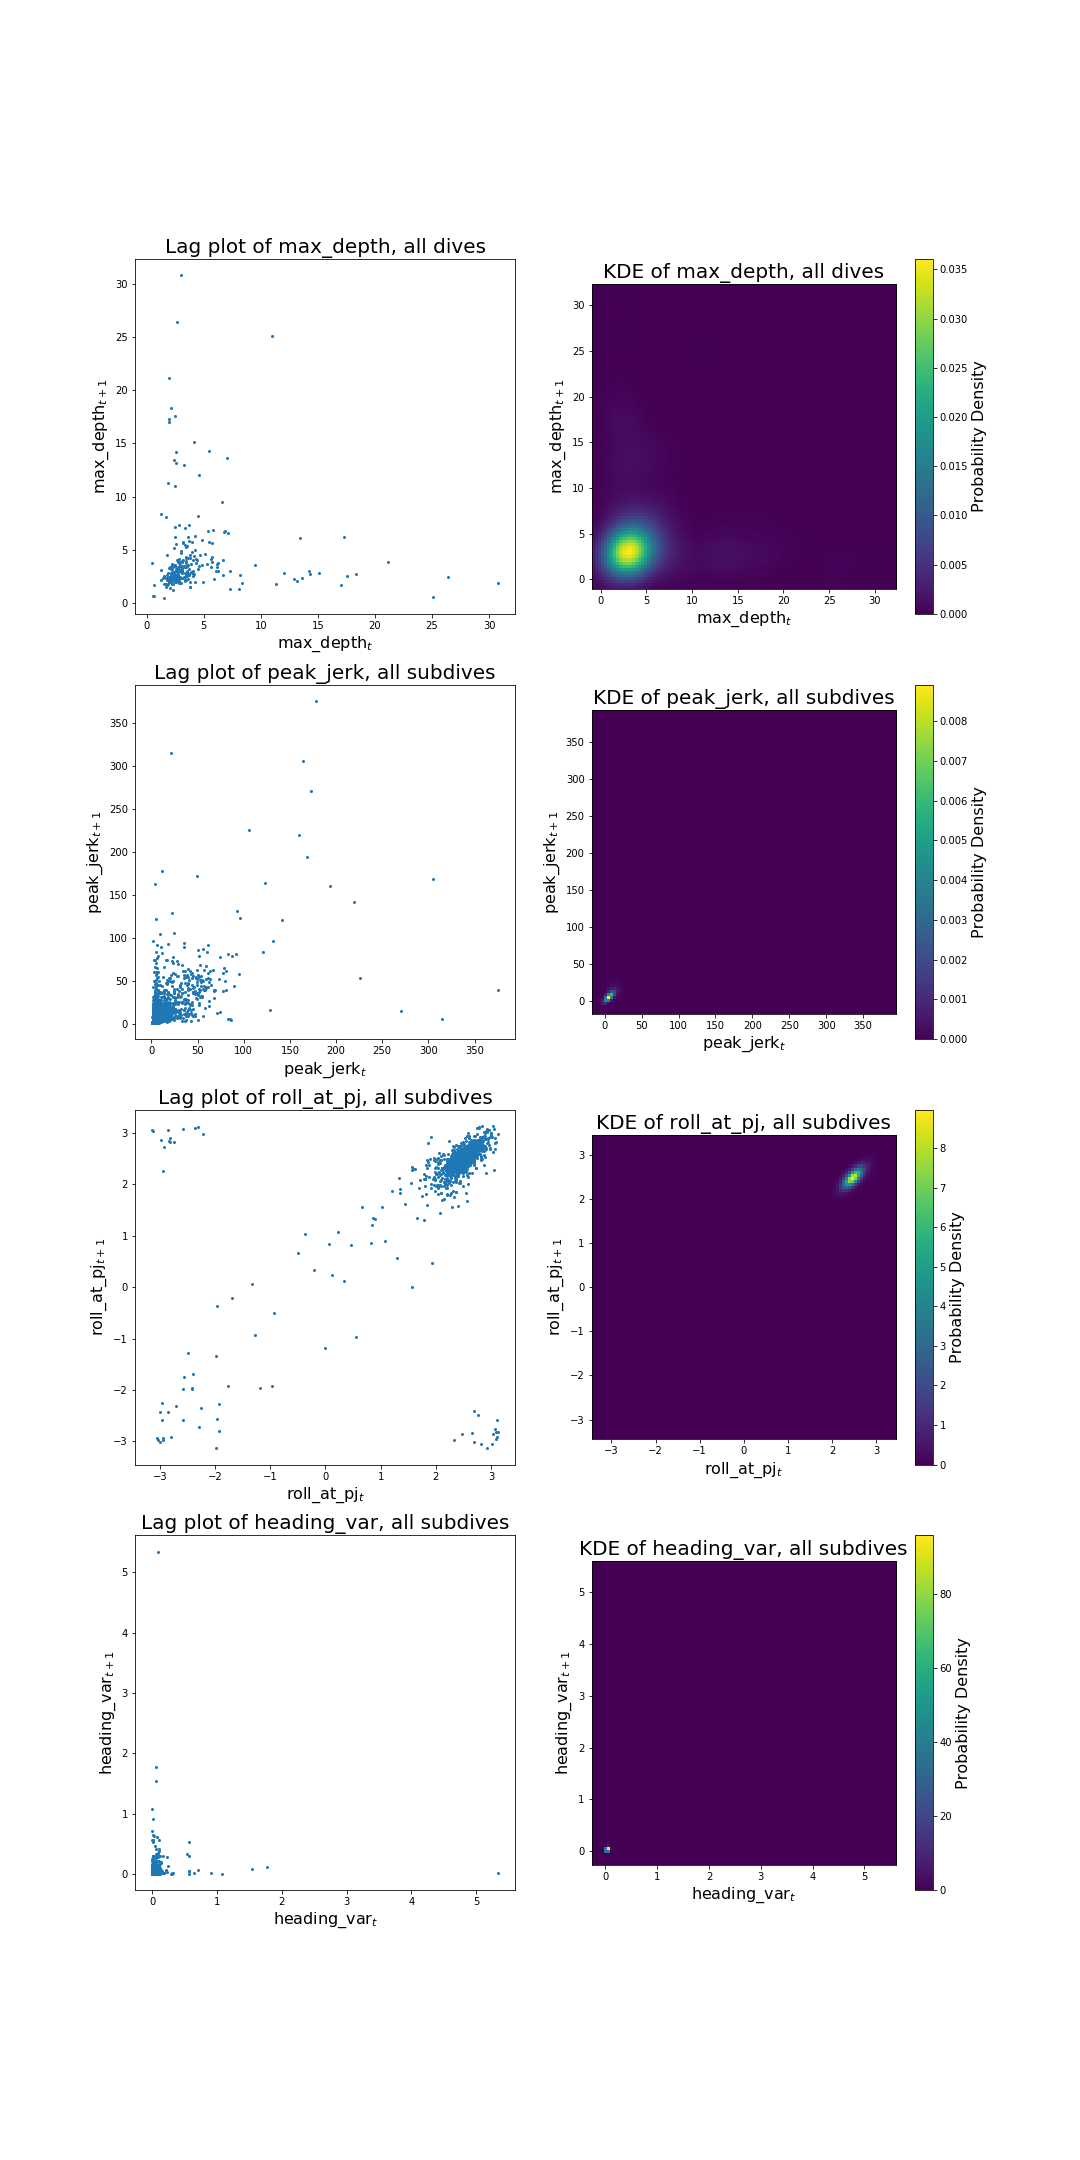
\includegraphics[height=7in]{../Plots/lagplot.png}
	\caption{Lag plot of all features (left) and the associated normal kernel density estimates (right)}
	\label{fig:lag}
\end{figure}

It is known that information criteria tends to overestimate the number of states in biological processes \citep{Pohle:2017}, so we instead selected $N = 2$ dive types and $N^* = 3$ sub-dive behaviours heuristically and admittedly somewhat arbitrarily. The absence of principled method to select the number of hidden states is a common issue in statistical ecology, so it is important to use model validation techniques in lieu of information criteria (see section \ref{subsec:model_validation}).

The final model is nearly identical to the one from the simulation study, with the exception that the fine scale Markov chain has three sub-dive behaviors instead of two ($N^* = 3$), and that $\mathbf{z}^{*(1)}_{t,t^*}$ is a vector rather than a scalar. The model is comprised of two levels: a coarse-scale HMM and a fine-scale CarHHMM-DFT. The coarse-scale model is comprised of an HMM with no auto-correlation and no DFT with hidden states corresponding to dive types and observations corresponding to dive durations. The fine-scale model is comprised of a CarHMM-DFT where auto-correlation is modeled into $\mathbf{z}^{*(1)}$ (the average acceleration with a 2-second window), but not $z^{*(2)}$ (the "wiggliness" of the 2-second window). Refer to (fig \ref{fig:CarHHMM}) for a graphical representation of this model.

\subsection{Results}

(Table \ref{table:emis_dists}) displays the emission distribution parameter estimates. Each distribution is also plotted in (fig \ref{fig:coarse_emis}) and (fig \ref{fig:fine_emis}).
%
\begin{figure}[ht]
	\centering
	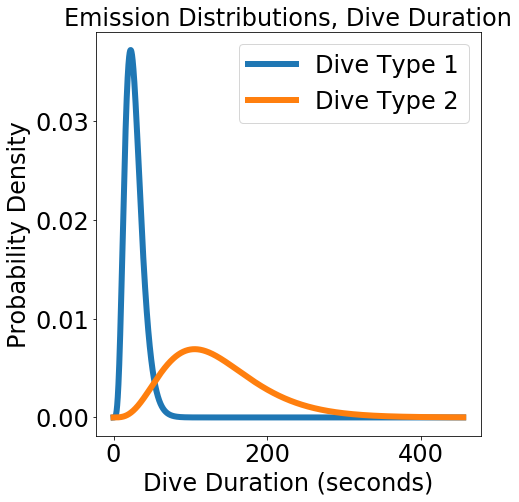
\includegraphics[height=4in]{../Plots/coarse-emissions.png}
	\caption{Estimated probability distributions for each coarse-scale observation in each dive type.}
	\label{fig:coarse_emis}
\end{figure}
%
\begin{figure}[ht]
	\centering
	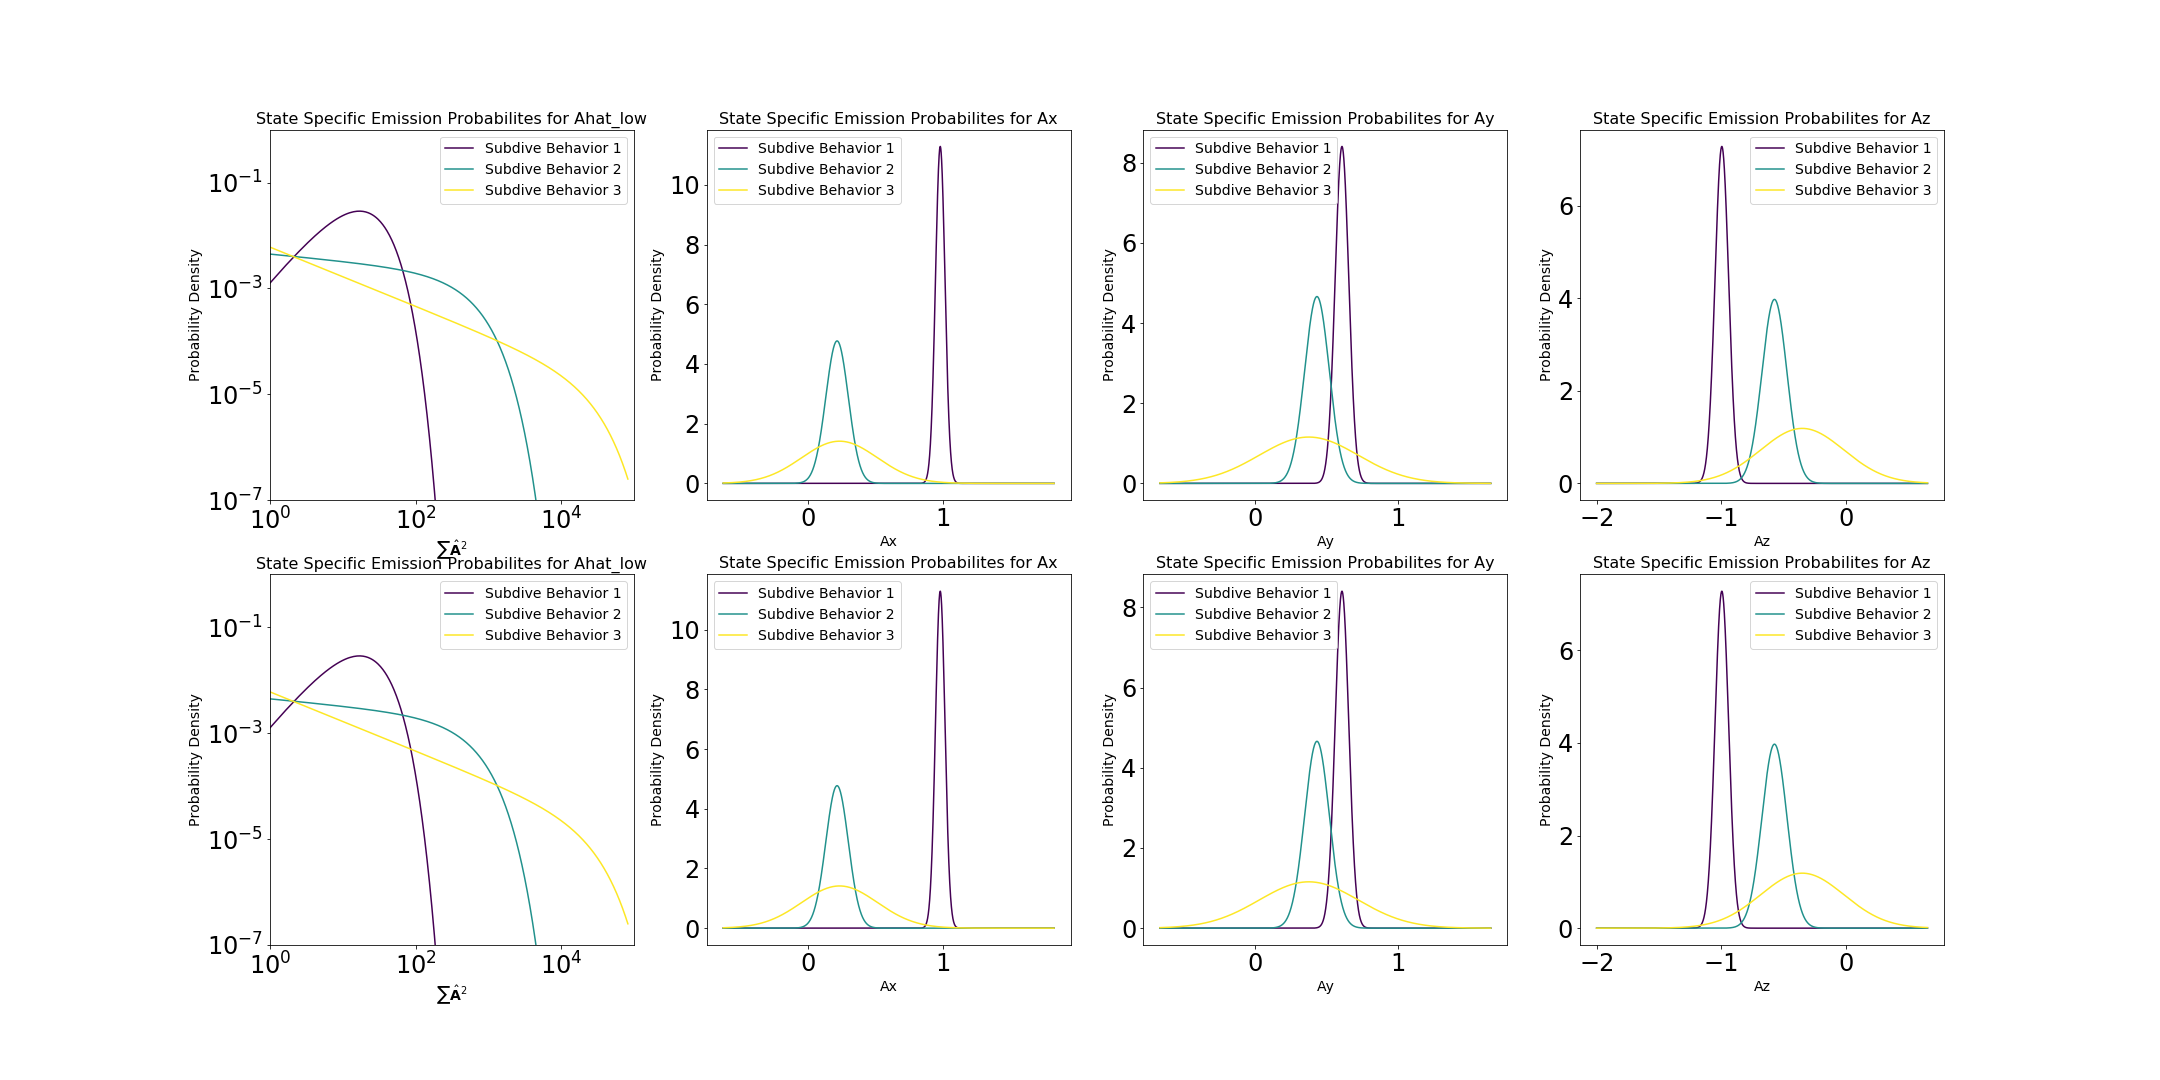
\includegraphics[height=2.5in]{../Plots/fine-emissions.png}
	\caption{Estimated probability distributions for each fine-scale observation in each behavioral state. Note that the distributions of acceleration do not take auto-correlation into account (see table \ref{table:emis_dists})}
	\label{fig:fine_emis}
\end{figure}
%
\begin{table}[ht]
    \centering
    \caption{Estimates and standard errors of emission parameters for killer whale data.}
    \scalebox{0.8}{
    \begin{tabular}{ccccc}
    \multirow{2}{*}{Feature}                 & \multirow{2}{*}{Dive / Sub-dive Type} & \multicolumn{3}{c}{Parameter Estimate}              \\
                                             &                                      & $\hat \mu$      & $\hat \sigma$   & $\hat \phi$     \\ \hline
    \multirow{2}{*}{Dive Duration (seconds)} & 1                                    & $27.23 \pm 0.63$ & $10.89 \pm 0.56$ & ---             \\
                                             & 2                                    & $127.96 \pm 11.50$ & $64.13 \pm 9.21$ & ---             \\ \hline
    \multirow{3}{*}{$Y^{*(1)}_x$}            & 1                                    & $0.98 \pm 0.07$ & $0.04 \pm 0.00$ & $0.99 \pm 0.00$ \\
                                             & 2                                    & $0.22 \pm 0.01$ & $0.08 \pm 0.00$ & $0.87 \pm 0.01$ \\
                                             & 3                                    & $0.23 \pm 0.03$ & $0.28 \pm 0.01$ & $0.62 \pm 0.03$ \\ \hline
    \multirow{3}{*}{$Y^{*(1)}_y$}            & 1                                    & $0.61 \pm 0.09$ & $0.05 \pm 0.00$ & $0.99 \pm 0.00$ \\
                                             & 2                                    & $0.43 \pm 0.01$ & $0.09 \pm 0.00$ & $0.87 \pm 0.01$ \\
                                             & 3                                    & $0.38 \pm 0.04$ & $0.35 \pm 0.01$ & $0.62 \pm 0.04$ \\ \hline
    \multirow{3}{*}{$Y^{*(1)}_z$}            & 1                                    & $-1.00 \pm 0.11$ & $0.05 \pm 0.00$ & $0.99 \pm 0.00$ \\
                                             & 2                                    & $-0.57 \pm 0.01$ & $0.10 \pm 0.00$ & $0.87 \pm 0.01$ \\
                                             & 3                                    & $-0.35 \pm 0.04$ & $0.34 \pm 0.01$ & $0.62 \pm 0.04$ \\ \hline
    \multirow{3}{*}{$Y^{*(2)}$}              & 1                                    & $27.16 \pm 0.32$ & $16.67 \pm 0.32$ & ---             \\
                                             & 2                                    & $406.98 \pm 4.42$ & $438.09 \pm 5.49$ & ---             \\
                                             & 3                                    & $9688.54 \pm 221.95$ & $14584.02 \pm 358.40$ & ---             \\ \hline
    \end{tabular}
    }
    \label{table:emis_dists}
\end{table}
%
While the ecological interpretation of behavioral states is tenuous for HMMs, we hypothesize the following meanings. Dive type 1 corresponds to shorter, shallower dives which serve a variety of purposes, including as rest before dives of type 2, which are deeper and more sustained. Sub-dive behavioural state 1 corresponds to gliding and less overall activity compared to the other behavioral states. The mean of $Z^{*(2)}$ in this state is at least an order of magnitude smaller than sub-dive behavior 2, the variance of $\mathbf{Z}^{*(1)}$ is smaller than sub-dive behavior 2 for every component, and the auto-correlation of $\mathbf{Z}^{*(1)}$ is higher than every other behavioral state. Sub-dive state 3, on the other hand, corresponds to vigorous swimming activity, as the mean of $Z^{*(2)}$ and variance of $\mathbf{Z}^{*(1)}$ for every component are much higher than every other state. The auto-correlation of $\mathbf{Z}^{*(1)}$ is also much lower in this state, implying more variation in acceleration every 2 seconds. Finally, sub-dive state 2 corresponds to a moderate amount of activity, as almost every parameter estimate is between the other two behavioral states.

The estimated probability transition matrices and associated stationary distributions are
%
$$\hat \Gamma = \begin{pmatrix} 
0.849 & 0.151 \\
0.907 & 0.093
\end{pmatrix}$$
$$\hat \delta = \begin{pmatrix} 0.857 & 0.143 \end{pmatrix}$$
%
$$\hat \Gamma^{*(1)} = \begin{pmatrix} 
0.724 & 0.276 & 0.000 \\
0.057 & 0.887 & 0.056 \\
0.000 & 0.247 & 0.753
\end{pmatrix} \qquad 
\hat \Gamma^{*(2)} = \begin{pmatrix} 
0.871 & 0.129 & 0.000 \\
0.135 & 0.829 & 0.036 \\
0.000 & 0.246 & 0.754
\end{pmatrix}$$
$$\hat \delta^{*(1)} = \begin{pmatrix} 0.143 & 0.698 & 0.159 \end{pmatrix} \qquad
\hat \delta^{*(2)} = \begin{pmatrix} 0.476 & 0.456 & 0.067 \end{pmatrix}$$.
%
About 86\% of observed dives are short- the whale usually rests for many dives in a row before performing a deep dive. The probability transition matrix $\hat \Gamma$ shows that the distribution of a particular dive's type is approximately equal regardless of the previous dive type. The fine-scale probability transition matrices imply that the killer whale is much more likely to be in a less active sub-dive state when performing deep dives than when performing shallow dives- 14\% of shallow dives are spent in sub-dive state 1 while 48\% of deep dives are spent in sub-dive state 1. Using less active sub-dive states when diving deep could be an energy reduction strategy for these long periods of holding breath- a phenomenon which has been observed in bottle-nose dolphins \citep{Williams:1999}. (Fig \ref{fig:labeled_dives}) shows the decoded dive behavior of 5 selected dives, and (fig \ref{fig:coarse_probs}) and (fig \ref{fig:fine_probs}) display the probability of each dive type and sub-dive state, respectively.

\begin{figure}[ht]
	\centering
	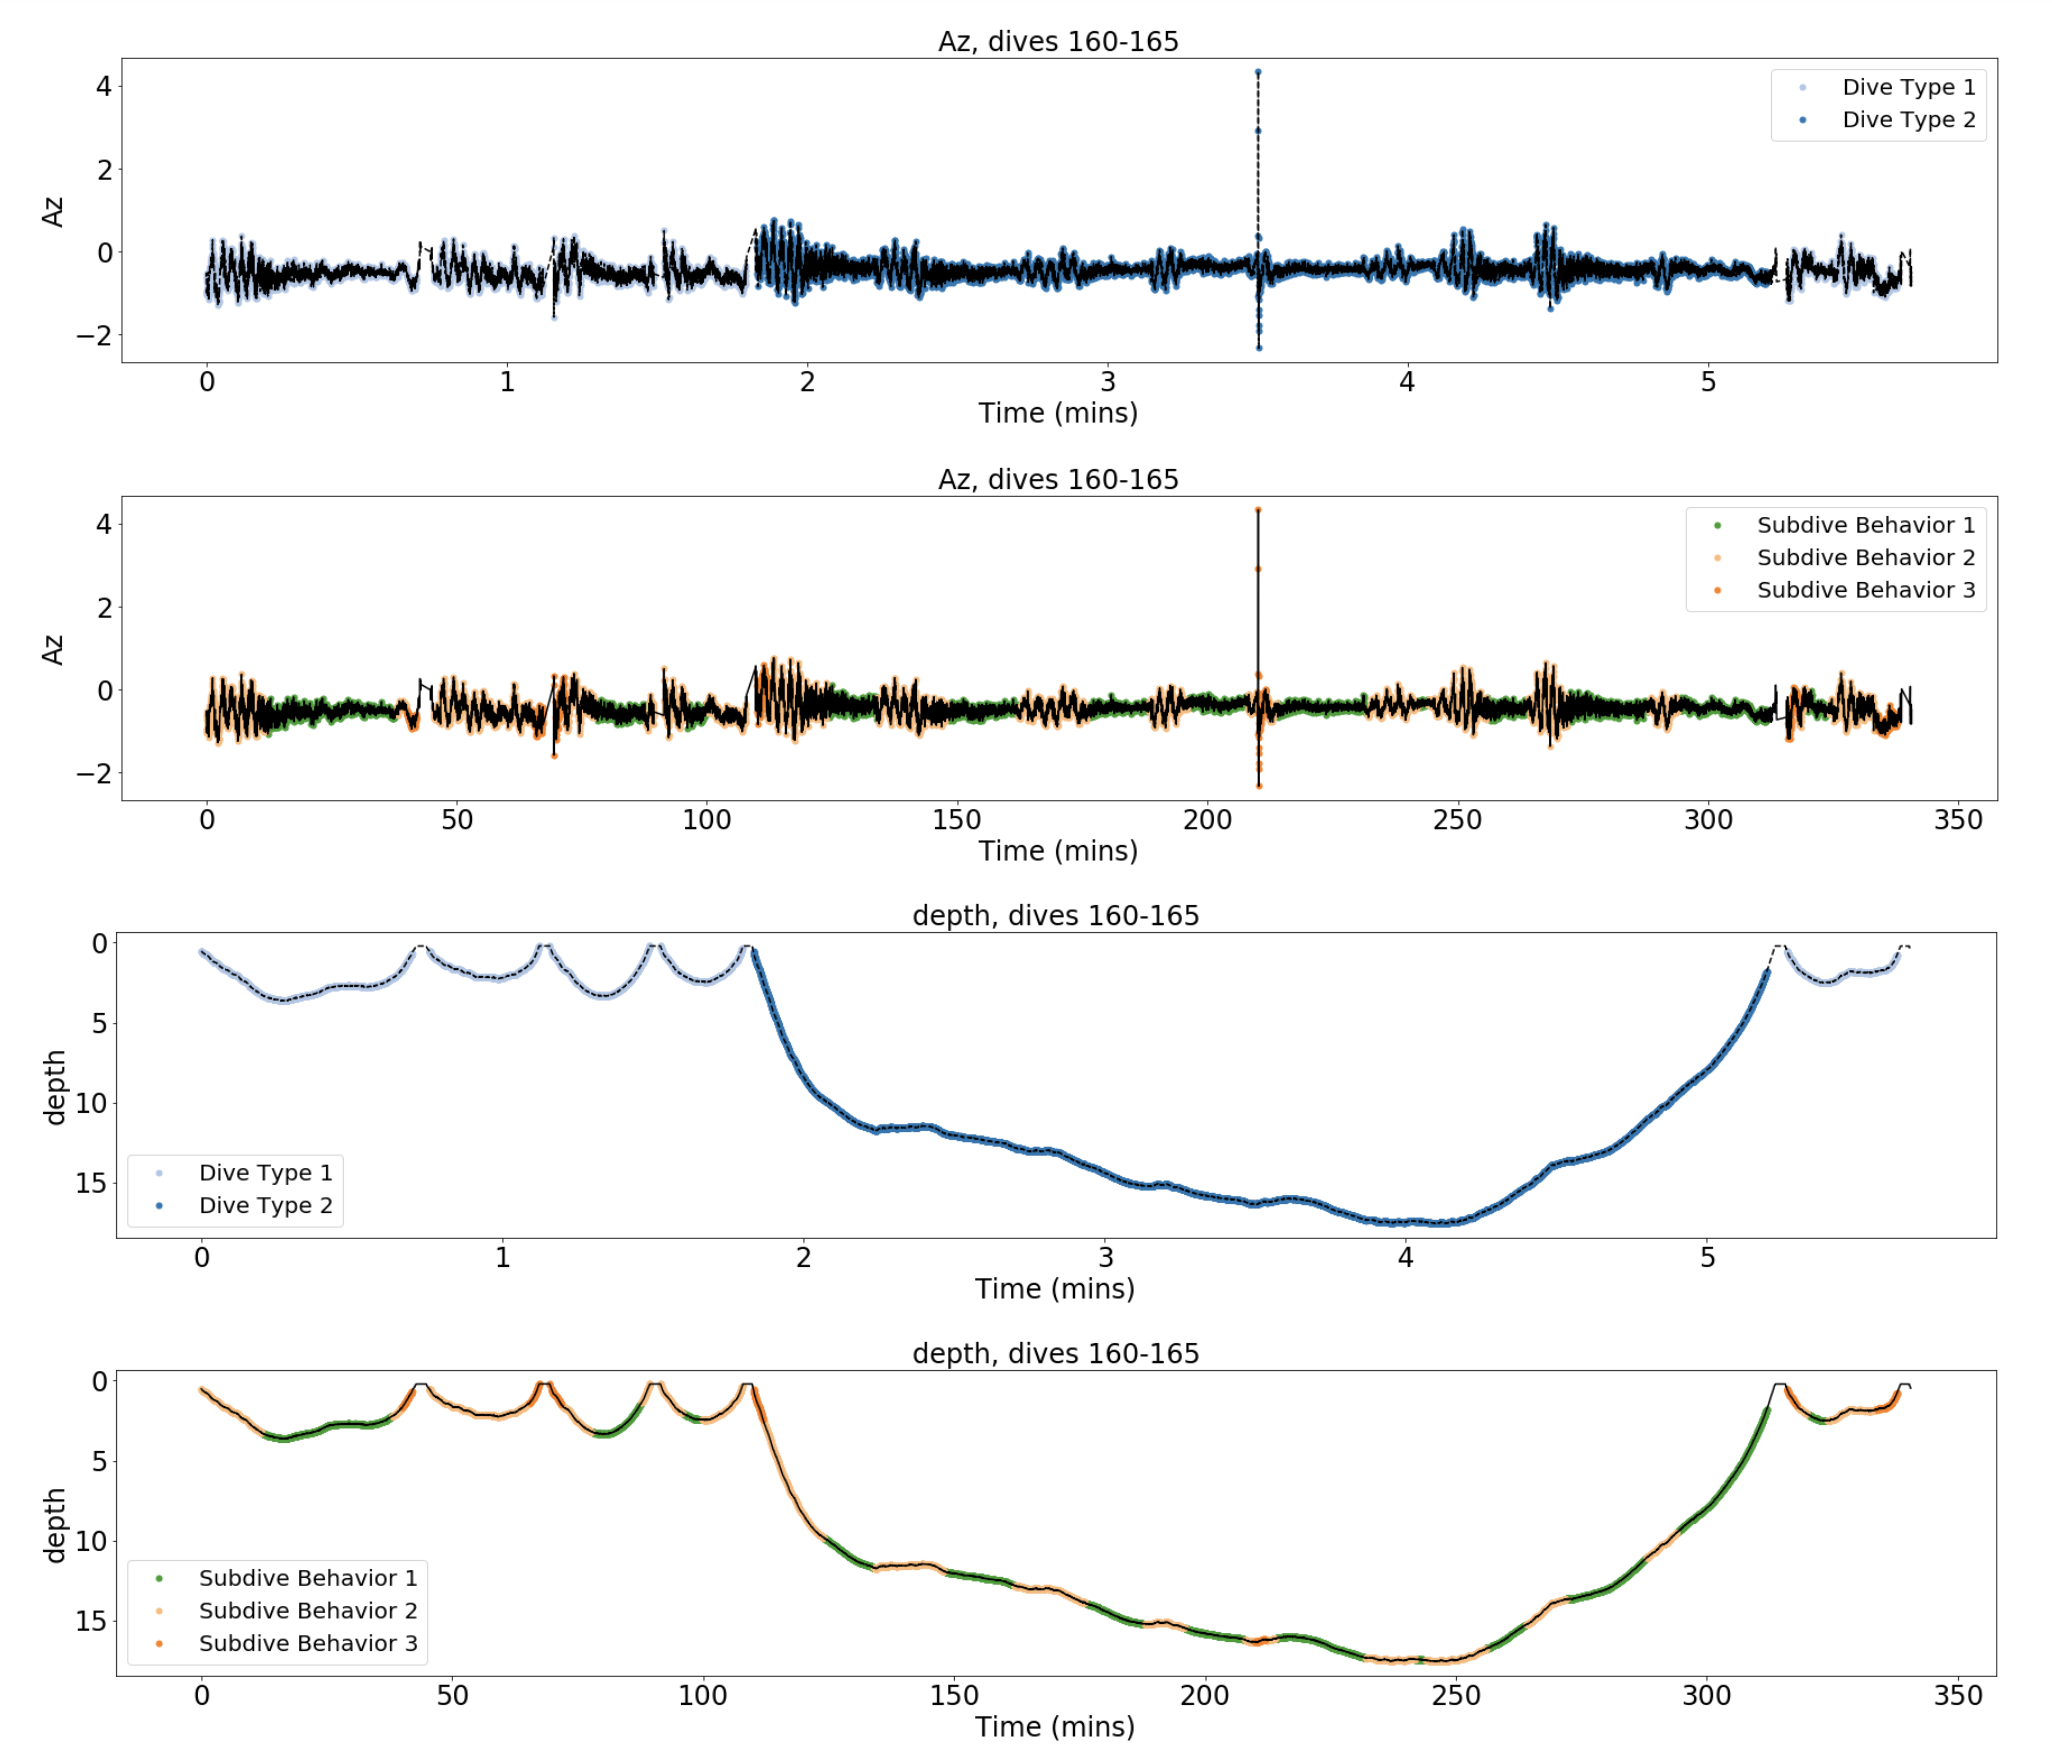
\includegraphics[width=5in]{../Plots/labeled_dives.png}
	\caption{Features of a particular set of killer whale dives and decoded estimates for the intra-dive behavioral states. The color of the plot corresponds to behavioral or dive state with the highest probability.}
	\label{fig:labeled_dives}
\end{figure}
%
\begin{figure}[ht]
	\centering
	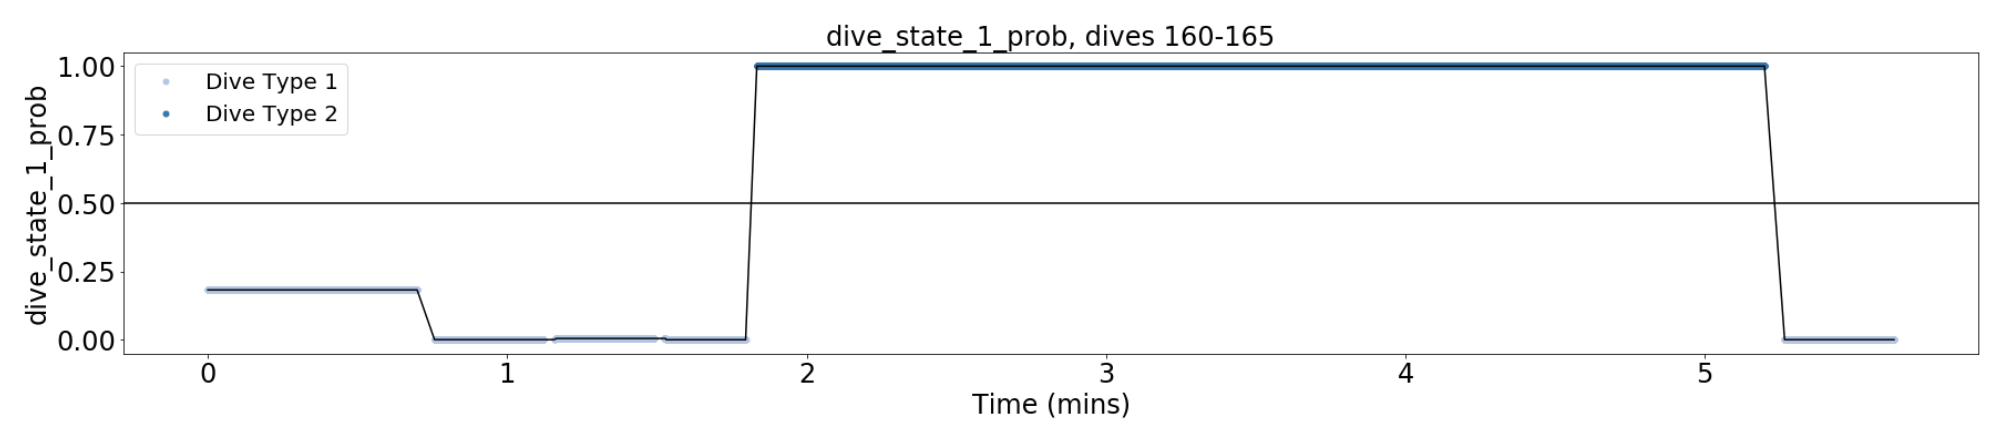
\includegraphics[width=5in]{../Plots/Coarse_state_probs.png}
	\caption{Probabilities of dive types for the set of killer whale dives from (fig \ref{fig:labeled_dives}).}
	\label{fig:coarse_probs}
\end{figure}
%
\begin{figure}[ht]
	\centering
	\begin{subfigure}[t]{1.0\textwidth}
        \centering
        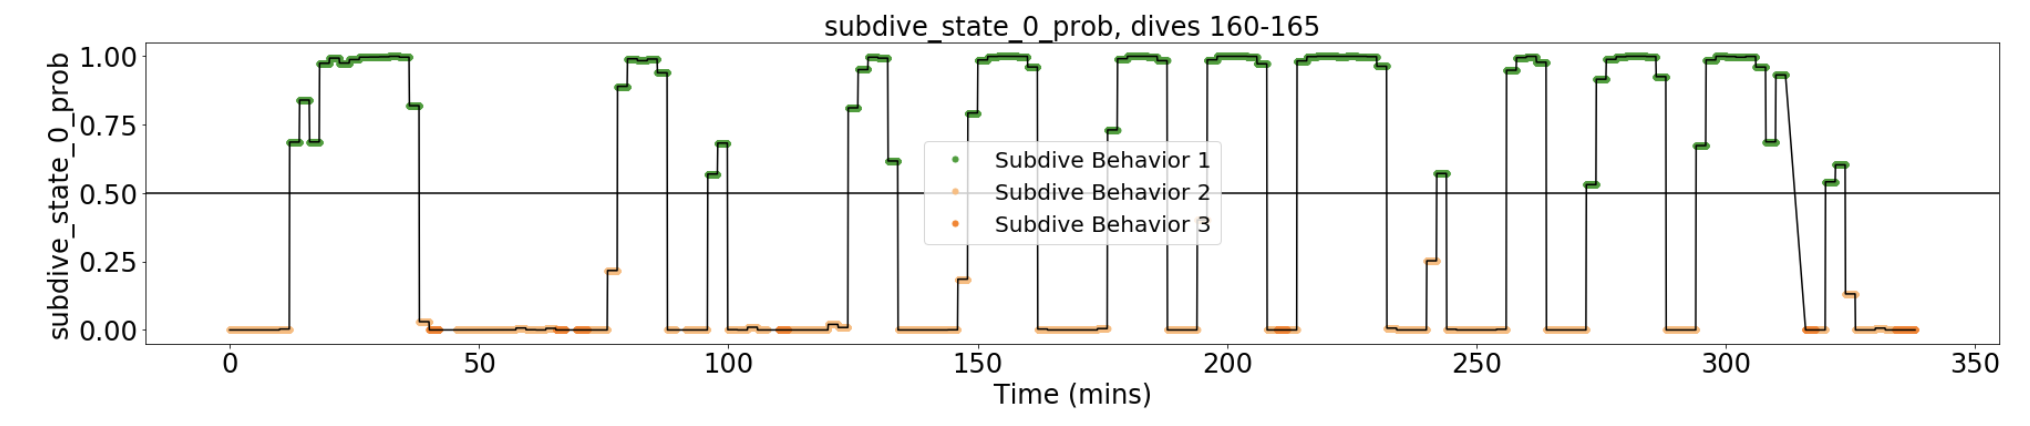
\includegraphics[width=5in]{../Plots/Fine_state_probs_1.png}
        \caption{Fine-scale state 1 probabilities}
    \end{subfigure}
    \newline
    \begin{subfigure}[t]{1.0\textwidth}
        \centering
        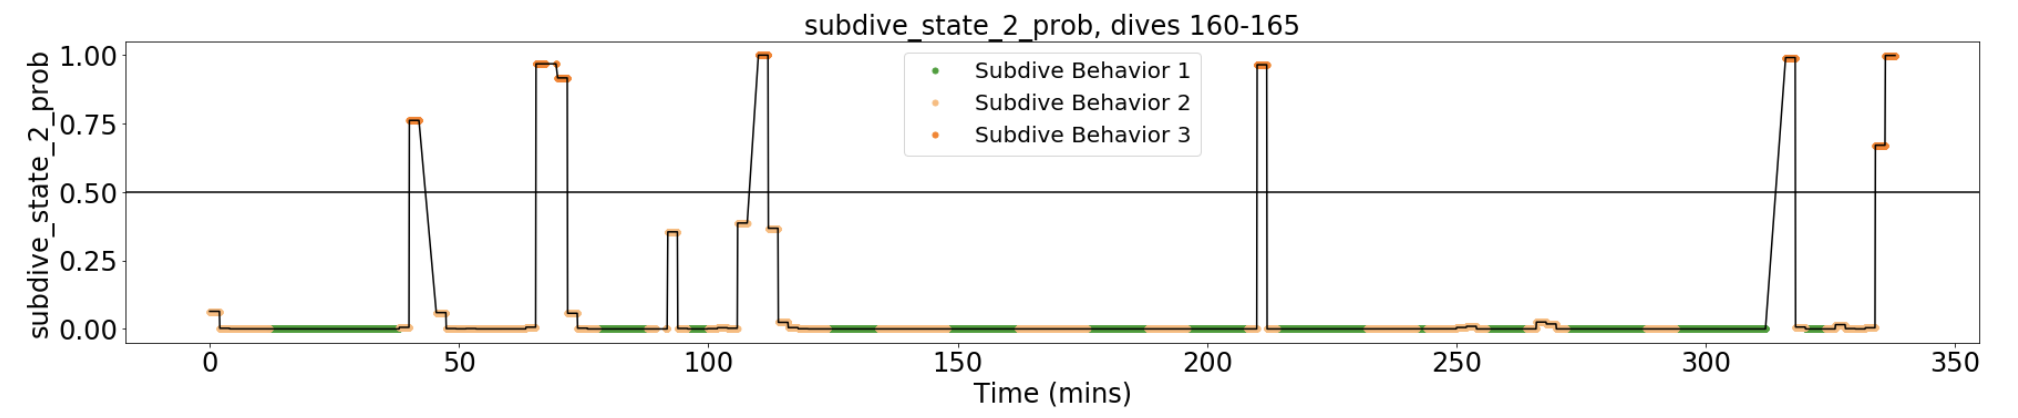
\includegraphics[width=5in]{../Plots/Fine_state_probs_3.png}
        \caption{Fine-scale state 3 probabilities}
    \end{subfigure}
	\caption{Probabilities of sub-dive types for the set of killer whale dives from (fig \ref{fig:labeled_dives}).}
	\label{fig:fine_probs}
\end{figure}

\subsection{Model Validation}
\label{subsec:model_validation}

Two visual tools were used to evaluate this model: pseudo-residuals and empirical histograms. A pseudo-residual of a particular observation is the marginal cdf of an observation conditioned on all other observations under the learned model \citep{Zucchini:2016}. To easily visualize outliers, the pseudo-residual is often passed through the quantile function of the standard normal distribution. In particular, the pseudo-residual of an observation $y_t$ is $\Phi^{-1} \left(Pr(Y_t < y_t|\{Y_1,\ldots,Y_T\}/\{Y_t\}) \right)$, where $\Phi$ is the cumulative distribution function of a standard normal distribution. If the model is correct, then all pseudo-residuals should be independent and follow a standard normal distribution. We find that histograms of the pseudoresiduals mostly support that the model is well-specified. $Z^{*(2)}$ is a notable exception, as its pseudo-residuals are noticeably right-skewed (fig \ref{fig:pseudoresids}). This implies that the true distribution of $Z^{*(2)}$ may follow a heavier-tailed distribution compared to a gamma distribution such as a power law. 

\begin{figure}[ht]
	\centering
	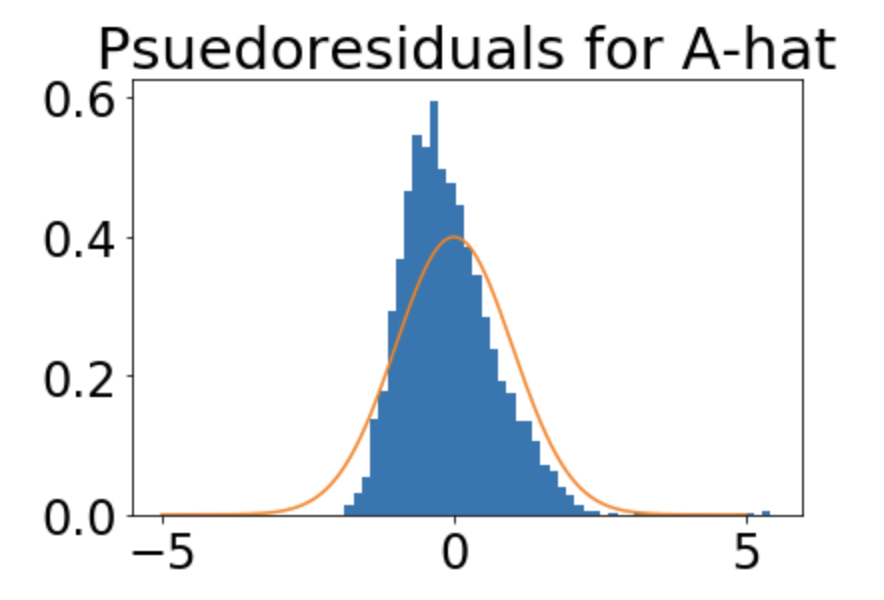
\includegraphics[width=5in]{../Plots/pseudoresids.png}
	\caption{Psuedoresiduals of $Y^{*(2)}$}
	\label{fig:pseudoresids}
\end{figure}

In addition to psuedoresiduals, we plot histograms of observations, weighted by the probability that the whale was in a particular hidden state. This empirical distribution was then plotted over the fitted probability distribution function of that feature and behavioral state. Our results mostly support a well-specified model with the exception of $Z^{*(2)}$, which is right-skewed. In addition, $\mathbf{Z}^{*(1)}$ has heavy tails for sub-dive state 3 (\ref{fig:empirical_dist}), indicating the existence of rare events corresponding to very violent trashing of the killer whale. These outliers are potential subjects for future study.

\begin{figure}[ht]
	\centering
	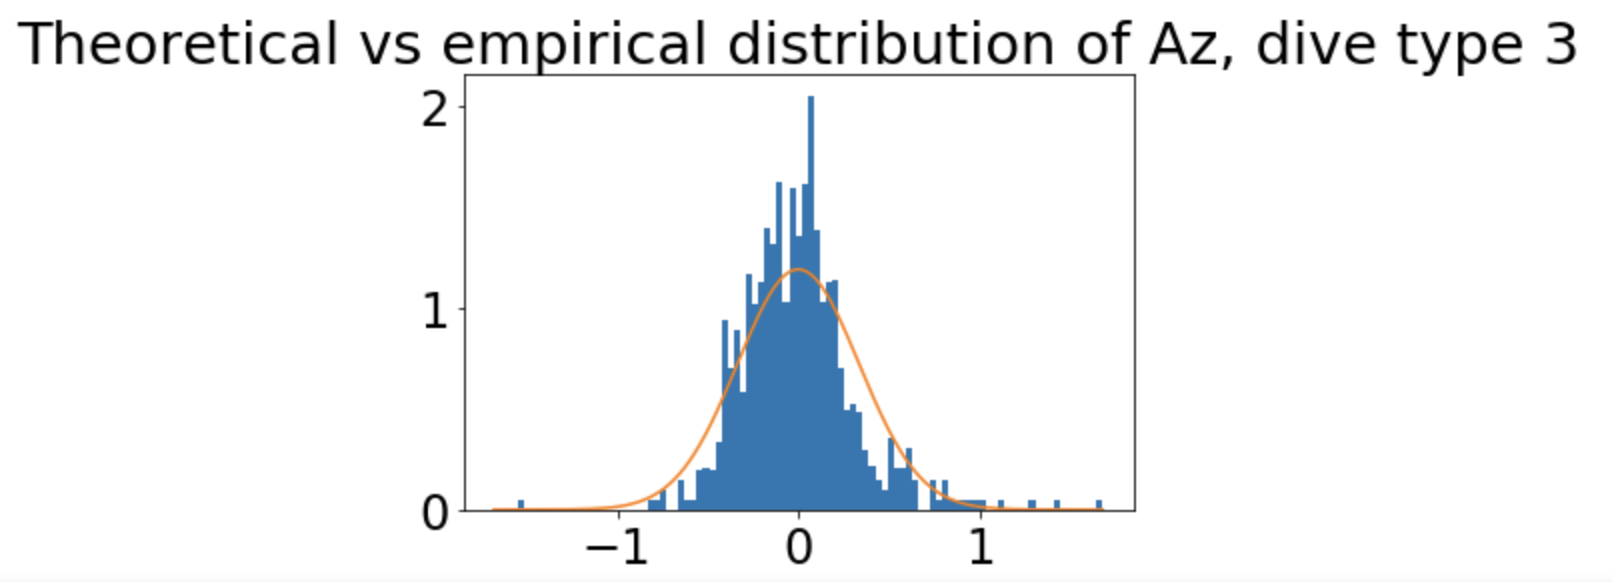
\includegraphics[width=5in]{../Plots/empirical_dist.png}
	\caption{Empirical distribution of $Y^{*(1)}_z$ for sub-dive state 3 plotted over its estimated pdf.}
	\label{fig:empirical_dist}
\end{figure}